\documentclass[11pt]{article}
% ---------------------------------------------------------------------------
%  ccint project wrap-up — preamble
%  Compiles with pdfLaTeX (Overleaf default; no configuration needed).
% ---------------------------------------------------------------------------
\usepackage[T1]{fontenc}
\usepackage[utf8]{inputenc}
\usepackage{lmodern}
\usepackage[letterpaper,margin=1in,headheight=14pt]{geometry}
\usepackage{microtype}
\setlength{\emergencystretch}{3em}   % 允许必要时额外伸缩，消除长代码标识符造成的溢出

\usepackage{booktabs}
\usepackage{tabularx}
\usepackage{longtable}
\usepackage{array}
\usepackage{multirow}
\usepackage{amssymb}
\usepackage{amsmath}
\usepackage{enumitem}
\usepackage{fancyhdr}
\usepackage{titlesec}
\usepackage{graphicx}
\graphicspath{{figures/}}
\usepackage{tikz}
\usetikzlibrary{arrows.meta,positioning,calc,fit,backgrounds}
\usepackage[skins,breakable]{tcolorbox}

\usepackage[dvipsnames]{xcolor}
\definecolor{ink}{HTML}{1A1A1A}
\definecolor{accent}{HTML}{1F4E79}
\definecolor{warn}{HTML}{9C4221}
\definecolor{good}{HTML}{22543D}
\definecolor{rule}{HTML}{C8CDD4}
\definecolor{softbg}{HTML}{F4F6F8}
\definecolor{accentbg}{HTML}{EAF0F6}

\usepackage[font=small,labelfont={bf,color=accent},skip=8pt]{caption}

\usepackage[colorlinks=true,linkcolor=accent,urlcolor=accent,citecolor=accent]{hyperref}

% --- headers ---------------------------------------------------------------
\pagestyle{fancy}
\fancyhf{}
\renewcommand{\headrulewidth}{0.4pt}
\fancyhead[L]{\footnotesize\textcolor{accent}{ccint — Canada Cyber Social Intelligence}}
\fancyhead[R]{\footnotesize\thepage}

% --- section styling -------------------------------------------------------
\titleformat{\section}{\Large\bfseries\color{accent}}{\thesection}{0.7em}{}
\titleformat{\subsection}{\large\bfseries\color{ink}}{\thesubsection}{0.6em}{}
\titleformat{\subsubsection}{\normalsize\bfseries\itshape\color{ink}}{}{0em}{}
\titlespacing*{\section}{0pt}{2.2ex plus 1ex minus .2ex}{1.2ex plus .2ex}

% --- table helpers ---------------------------------------------------------
\renewcommand{\arraystretch}{1.18}
\newcolumntype{R}{>{\raggedleft\arraybackslash}X}
\newcolumntype{L}{>{\raggedright\arraybackslash}X}
\newcommand{\hd}[1]{\textbf{#1}}

% --- callout boxes ---------------------------------------------------------
\newtcolorbox{keybox}[1][]{
  enhanced, breakable, colback=accentbg, colframe=accent,
  boxrule=0pt, leftrule=3pt, arc=1pt, left=8pt, right=8pt, top=6pt, bottom=6pt,
  #1}
\newtcolorbox{warnbox}[1][]{
  enhanced, breakable, colback=softbg, colframe=warn,
  boxrule=0pt, leftrule=3pt, arc=1pt, left=8pt, right=8pt, top=6pt, bottom=6pt,
  #1}
\newtcolorbox{plainbox}[1][]{
  enhanced, breakable, colback=softbg, colframe=rule,
  boxrule=0.4pt, arc=1pt, left=8pt, right=8pt, top=6pt, bottom=6pt,
  #1}

% --- inline semantics ------------------------------------------------------
\newcommand{\code}[1]{\texttt{\small #1}}
\newcommand{\yes}{\textcolor{good}{\checkmark}}
\newcommand{\no}{\textcolor{warn}{$\times$}}
\newcommand{\noise}{\textcolor{warn}{noise}}

% --- verbatim-ish code block ----------------------------------------------
\usepackage{fancyvrb}
\DefineVerbatimEnvironment{shell}{Verbatim}
  {fontsize=\small,frame=single,rulecolor=\color{rule},framesep=6pt,
   formatcom=\color{ink}}


\title{\vspace{-1.6cm}\textbf{\color{accent}What the Instrument Can See}\\[2pt]
\large\color{ink} Measuring the coverage boundary of a social-media
cybersecurity sensor}
\author{\normalsize ccint --- iteration report}
\date{\normalsize 22 September 2026}

\begin{document}
\maketitle
\thispagestyle{fancy}
\vspace{-0.8cm}

\begin{keybox}
\textbf{In one paragraph.} The previous phase of this project established, by
permutation test, that no topic trend in the corpus is distinguishable from
noise, and measured that roughly eight times the data would be needed before
one could be. That leaves an obvious question: is the absence in the world or
in the instrument? This iteration built the measurements needed to answer it,
and the answer is specific. For the one event class we can verify against an
external registry --- Canadian ransomware victims --- the platform carries the
events almost perfectly (26 of 27) and the collector captures almost all of
what it carries (26 of 27), but essentially none of it is human discussion:
144 relevant posts from 15 accounts, of which three accounts and five posts
are not automated feeds, and all five concern a single event. What looked like
coverage is syndication. The corpus is a near-complete mirror of a handful of
threat-intelligence bots and a near-empty record of Canadian public attention
to cyber incidents.
\end{keybox}

\section{The question this iteration answers}

The system collects Canada-related cybersecurity discussion from Bluesky,
labels it under versioned schemes, and looks for temporal change. Its
headline result so far is negative and well-characterised: the largest
topic movement in the 30-day window, \code{data\_breach} at $+22\%$, has
$p_{\mathrm{FWER}} = 0.734$ under an author-level circular-shift null, and the
measured power requirement is about $8\times$ the current volume.

A negative result of that kind is only interesting if you know what produced
it. Three explanations were open:

\begin{enumerate}[leftmargin=1.4em,itemsep=2pt]
\item \textbf{The world.} Canadian cyber discussion genuinely has no structure
      at this timescale.
\item \textbf{The gate.} The relevance judge is too strict, so the corpus is a
      biased subsample of what was collected.
\item \textbf{The boundary.} The collector never retrieved the relevant
      material in the first place, so no judge could recover it.
\end{enumerate}

Nothing in the system could separate these, because every number it produced
came from labels it had produced itself. This iteration added the three
measurements that can, and they resolve in an order that was not the expected
one.

\section{What was measured}

\subsection{The collection boundary had never been examined}

The collector issues one search per term over a fixed list of 34
cybersecurity terms --- 25 English, 9 French --- and merges the results. None
of the 34 mentions Canada. The list has not changed since the first day of the
project; the \code{query\_version} mechanism faithfully recorded that it was
\code{cyber\_v1}, which guarantees reproducibility but says nothing about
adequacy.

Because Bluesky search is close to text matching, per-term productivity can be
reconstructed offline from the 91{,}551 posts already stored, without new
collection. Figure~\ref{fig:terms} plots what each term cost against what it
returned.

\begin{figure}[htbp]\centering
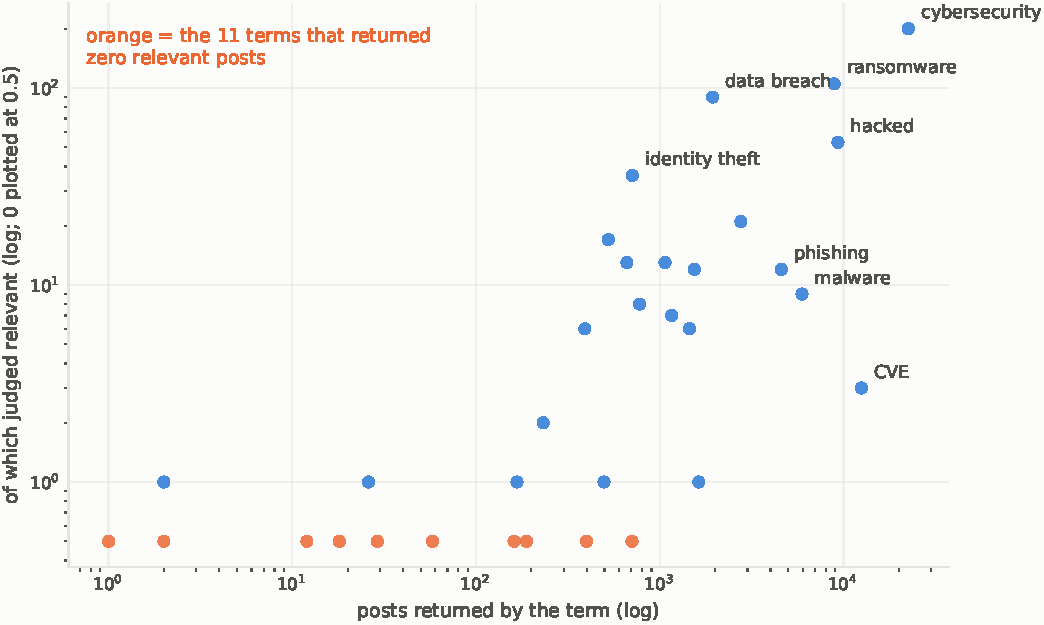
\includegraphics[width=\linewidth]{iter_terms.pdf}
\caption{Each search term: posts retrieved against posts subsequently judged
relevant. Both axes are logarithmic; terms with zero relevant posts are drawn
at $0.5$ so they remain visible. The distribution is not merely uneven --- it
is close to degenerate.}
\label{fig:terms}
\end{figure}

Three properties matter more than the ranking:

\begin{itemize}[leftmargin=1.4em,itemsep=2pt]
\item \code{CVE} retrieved 12{,}502 posts and yielded 3 relevant ones, a
      precision of $0.024\%$. It accounts for $13.7\%$ of everything collected.
\item Eleven terms returned zero relevant posts. One of them, \code{maliciel},
      returned no posts at all in 30 days.
\item \code{cybersecurity} alone accounts for $30.8\%$ of all relevant posts
      and $24.6\%$ of the entire corpus. The time series of the corpus is,
      to first order, the time series of one search term. Nothing monitors it.
\end{itemize}

\begin{warnbox}
The instructive part is the provenance. The project's specification named four
term pairs and wrote ``etc.''; the remaining 26 terms were supplied during
implementation from general domain knowledge. They were never derived from
data, never compared against an external list, and never revised. The
published work that does this well does one of two things: it inherits a list
from practitioners --- Tweezers (NDSS 2025) takes its keywords from a threat
intelligence company's analysts --- or it grows one from a seed by measured
expansion. Tweezers also reports what such lists cost: comparing its own
against the earlier W2E list, more than half of the tweets it collected would
have been missed by W2E, and W2E was itself missing \code{phishing},
\code{cve} and \code{patch}. Two lists built by professionals disagreed by more
than half.
\end{warnbox}

\subsection{The relevance gate, replaced and then measured}

The old gate was
\code{is\_relevant = has\_cyber\_term AND has\_canada\_term AND corroborated}.
Both sides are narrow instruments joined by a conjunction, so recall is
bounded by their intersection: of 91{,}551 posts collected, 650 passed
($0.72\%$), and the 89{,}714 rejected had never been examined by anything
semantic.

The replacement asks a model two questions, and the first design decision was
to keep them apart. A single prompt asking whether a post is about
\emph{cybersecurity in Canada} produced a $6.8\%$ pass rate on rejected posts,
and inspection showed why: the model had collapsed the conjunction onto the
side it knows better. The passing posts were Fortinet advisories, Lynx victim
listings, and a French story about the French Ministry of Education. Asked as
two independent questions, the Canadian side passed $1.08\%$, and the passing
posts began to include material that should have been there all along --- a
Quebec cabinet minister responsible for cybersecurity, \code{.ca} law-firm
domains, ``GC website'' as colloquial shorthand for the federal government.

A second decision follows from the corpus rather than from the model: ask
about Canada first, over everything, and ask about cyber only where a Canadian
entity was found. Every post in this corpus arrived through a cybersecurity
search term, so the cyber side is nearly always true and carries little
information; the Canadian side is the rare and binding one. Running it this
way also produces an entity map of the whole corpus as a by-product, which is
the input to query expansion and to event linking, and it reduces the call
count from $2N$ to $N + \varepsilon N$.

\paragraph{The gate's own failure, and its ceiling.}
The first version of the entity prompt recovered Canadian entities in only
$55.4\%$ of registry-verified positive posts --- and, more diagnostically, in
only $69.0\%$ of posts that contain the literal string \emph{Canada} or
\emph{Canadian}. Specificity was excellent at $99.5\%$. The failure was
therefore recall, and its cause was the prompt: a clause instructing the model
that an empty list is the expected answer, followed by a long list of
prohibitions, drove a 4B model to the null answer. Removing the restraint
clause and adding an explicit rule --- if the country name appears literally,
it counts --- moved literal-mention recall from $69.0\%$ to $99.3\%$
(Figure~\ref{fig:prompt}).

\paragraph{And the fix broke something the evaluation could not see.}
The corrected prompt raised corpus relevance from 906 posts to 3{,}528. That
number is wrong. Inspection of the additions found \code{trustedsec.com},
\code{malwarebytes.com}, the UK's \code{NCSC}, \code{Revolut}, a French story
about the \emph{\'Education nationale}, and \code{ia.cr} --- the Costa Rican
top-level domain. The prompt's clause \emph{``a \code{.ca} or \code{.gc.ca}
domain''} had been generalised by the model into \emph{``a domain''}.

Two mechanical checks, requiring no further model calls, quantify it:

\begin{center}
\begin{tabularx}{\linewidth}{@{}Lrr@{}}
\toprule
\hd{Extracted entity type} & \hd{Count} & \hd{Not present in the post text} \\
\midrule
\code{place}         & 2{,}192 & \textbf{1{,}053 \;(48.0\%)} \\
\code{org}           & 1{,}364 & 12 \;(0.9\%) \\
\code{domain}        & 1{,}296 & 49 \;(3.8\%) \\
\code{gov}           & 889     & 10 \;(1.1\%) \\
\midrule
\multicolumn{3}{@{}l}{\small Of the 1{,}296 \code{domain} entities, 312
($24.1\%$) actually end in a Canadian TLD.} \\
\bottomrule
\end{tabularx}
\end{center}

\begin{keybox}
\textbf{A verification channel obtained by accident.} Character offsets are
computed with \code{str.find} rather than requested from the model, on the
narrow grounds that small models miscount offsets. That decision turned into an
independent hallucination detector: an entity string that cannot be located in
the post was invented. Nearly half of all \code{place} entities were ---
the model writing ``Canada'' into a French post about a French ministry.
Declining to trust a model with a task it does badly produced a free check on
the task it was actually given.
\end{keybox}

Applying both rules --- discard entities absent from the text, discard domains
outside Canadian TLDs --- removes 2{,}086 entities and 1{,}180 posts, and
leaves the picture below. The validation layer is retained in the labeler even
though the prompt will be corrected, because it is deterministic, costs
nothing, and catches exactly the class of error the external evaluation set
cannot.

\begin{center}
\begin{tabularx}{\linewidth}{@{}Lrrr@{}}
\toprule
\hd{Relevance gate} & \hd{recall} & \hd{specificity} & \hd{corpus} \\
 & \hd{@\,registry pos.} & \hd{@\,registry neg.} & \hd{relevant} \\
\midrule
\code{rules\_v2} --- keyword conjunction       & 46.5\% & 99.8\% & 650 \\
\code{llm\_v2a} --- two questions, prompt v1   & 53.5\% & 99.7\% & 860 \\
\code{llm\_v2c} --- prompt v2 + validation     & \textbf{68.3\%} & 99.4\% & \textbf{2{,}348} \\
\midrule
\multicolumn{4}{@{}l}{\small \emph{before} validation, prompt v2 reported
$69.3\%$ / $99.0\%$ / 3{,}528 --- one third of that corpus was spurious.} \\
\bottomrule
\end{tabularx}
\end{center}

\begin{warnbox}
\textbf{The negative set certified a corpus that was a third wrong.} A
specificity of $99.0\%$ on \code{E\_reg\_neg} implies roughly 890 false
positives across 89{,}044 posts. The true figure was 1{,}181. The negative set
did not detect the failure because it is composed of feed posts about foreign
ransomware victims: formulaic English, few URLs, no French. The model's actual
failure modes --- over-generalising a domain rule, hallucinating a country name
into French text --- do not occur in that population. An external label removes
self-reference; it does not confer representativeness, and a non-representative
evaluation set does not merely fail to detect a regression, it actively
certifies one.
\end{warnbox}

\paragraph{What remains is a knowledge ceiling.}
Of the posts the corrected and validated extractor still misses, \textbf{none}
contains the word \emph{Canada} in any form. They read \emph{``New post from
\#Qilin: Coldfish Seafood''} --- a real Canadian victim, named, with no country
marker anywhere in the text. No amount of prompting will let a 4B model know
that Coldfish Seafood is Canadian.

\begin{keybox}
This is a ceiling of a particular kind. The residual error in the relevance
gate is not a model-capability problem and not a prompt problem: it is missing
world knowledge about small Canadian organisations. The only thing that
resolves it is a gazetteer --- and the gazetteer that would resolve it is the
external registry currently being used to measure the gap. The measurement
instrument and the repair are the same object.
\end{keybox}

\subsection{An external reference, and what it revealed about itself}

Until this iteration every precision and recall figure in the project traced
back to a single author: the person who wrote the rules also wrote the
prompts and produced the hand-coded evaluation set. A reported $\kappa = 0.870$
measures agreement under those conditions, not independence.

The registry breaks that loop. Victim records were ingested from
ransomware.live for Canada (positives) and the United States, France and the
United Kingdom (negative entity sources): 1{,}080 events and 1{,}943 entities.
Matching victim organisation names against the corpus produces evaluation sets
whose labels no part of this system produced.

Two constraints were imposed on their construction, and both turned out to
matter more than expected.

\emph{First, the definition of an evaluation set may not contain the output of
the system being evaluated.} A natural specification for the negative set was
``mentions a foreign victim, and \code{rules\_v2} judged \code{is\_canada}
false''. That specification makes \code{rules\_v2} precision identically $1$
on the set, and any replacement can only appear worse --- an artefact of
construction with no relation to capability. The negative set uses registry
conditions only.

\emph{Second, the positive set must be stratified by account type.} The reason
is visible in the data: registry victim names appear on Bluesky almost
exclusively inside the accounts that syndicate the registry. Of 101 positive
posts, 100 come from automated feeds; the three largest contributors are
\code{ransomlook}, \code{cyberintelligence} and \code{ransomware.live} itself.
Median engagement is zero and $94.9\%$ of the posts have no likes at all. The
single post classified as non-feed turned out to be a golf-industry content
farm auto-generating an article about a golf club's ransomware incident, with
zero likes, zero reposts and zero replies.

\begin{warnbox}
\textbf{A metric that rewards capturing bots.} Had \code{recall@E\_reg\_pos}
been adopted as the optimisation target, it would have climbed towards
$100\%$, because those posts are formulaic and a model need only learn that
``Inglewood Golf'' is a Canadian company. The metric would improve
substantially while the research question --- what Canadians say about cyber
incidents --- received no answer at all. External labels are necessary but not
sufficient: an external label attached to a non-independent \emph{population}
reintroduces the circularity it was meant to remove.
\end{warnbox}

\section{The central result}

Combining the registry with a targeted per-event search over the platform
separates the three explanations. For every Canadian event in the window, the
victim organisation's name was searched directly on Bluesky --- with no
cybersecurity term attached --- over a $[-2, +30]$ day window. Because bare
organisation names attract unrelated traffic (\emph{MEQ} retrieves the medical
unit; \emph{Air Canada} retrieves fare deals), every hit was then passed
through the cyber judgement before counting. This is entity-directed
retrieval: it establishes an upper bound on what the platform could have
yielded for an event whose identity is already known.

\begin{figure}[htbp]\centering
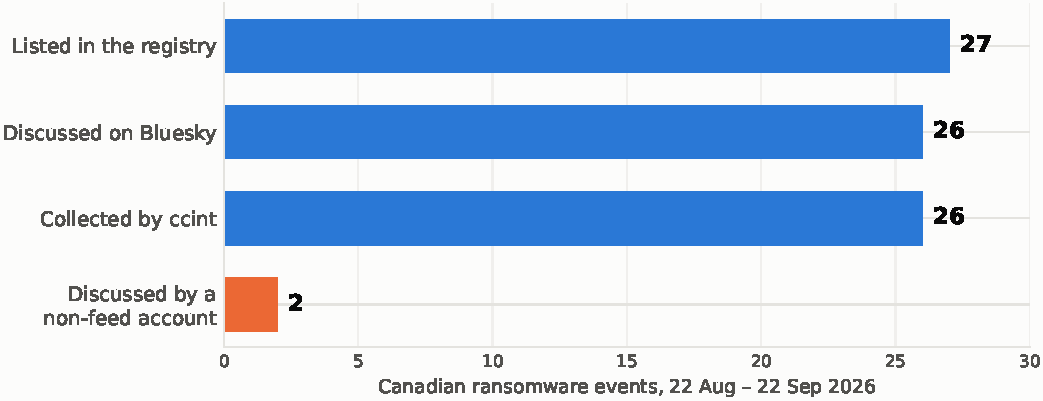
\includegraphics[width=\linewidth]{iter_funnel.pdf}
\caption{The same 27 Canadian ransomware events at four successive gates. The
attrition is almost entirely at the last one, and the last one is not a
property of this system.}
\label{fig:funnel}
\end{figure}

\begin{center}
\begin{tabularx}{\linewidth}{@{}Lrr@{}}
\toprule
\hd{Stage} & \hd{Events} & \hd{Share} \\
\midrule
Listed in the registry, in window & 27 & --- \\
At least one cyber-related post exists on Bluesky & 26 & 96\% \\
At least one such post was collected by ccint & 26 & 96\% \\
At least one such post came from a non-feed account & \textbf{2} & \textbf{7\%} \\
\bottomrule
\end{tabularx}
\end{center}

\medskip

The 144 cyber-related posts across these events come from 15 accounts. Twelve
are automated threat-intelligence feeds. The three that are not are Canadian
news organisations --- \code{ctvnewsmontreal}, \code{mediasca},
\code{985fm.ca} --- contributing five posts between them, all about the same
event. Individual users contributed nothing.

\begin{keybox}
\textbf{The collector is not the bottleneck for this event class.} It captured
26 of the 26 events the platform carried. The reason the corpus contains no
detectable trend in ransomware discussion is that there is almost no
ransomware \emph{discussion} to detect --- there is a nearly complete mirror of
several leak-site feeds, and the corpus reproduces it faithfully.
\end{keybox}

\subsection{The one event that behaved differently}

The exception is worth stating in full, because it is the only case in the
month where the platform behaved the way the project assumed it would.

The Commission de la construction du Qu\'ebec, a provincial construction
industry regulator, was listed by the Qilin ransomware group; roughly 350{,}000
people's data was taken. This event drew genuine Canadian media coverage on
Bluesky, in French and English: \code{ctvnewsmontreal} on a class action filed
in Quebec Superior Court, \code{mediasca} on Russian attackers taking the
records of 350{,}000 people, \code{lapresse.ca}, and \code{985fm.ca} carrying
an interview with the CCQ's chief executive.

Four of those five posts are in the corpus. The one that is not reads
\emph{``Une protection pr\'eventive mise en place \`a la CCQ: \guillemotleft Je
me sens responsable \guillemotright''}. It contains no term from the
34-term list --- \emph{protection pr\'eventive} is not in any lexicon --- and so
it was unreachable. This is the collection-boundary gap at human scale: one
post, one missing phrase, a real event, a real Canadian outlet.

\subsection{Two gaps, and a reference that can only see one}

The measurements point at two distinct deficiencies, and conflating them would
be a mistake.

\begin{center}
\begin{tabularx}{\linewidth}{@{}Lp{4.4cm}p{4.4cm}@{}}
\toprule
 & \hd{Registry-verifiable events} & \hd{General Canadian cyber talk} \\
\midrule
Collection recall & 26/27 events (96\%) & unmeasured; at least 901 rejected
posts carry a Canadian entity \\
Binding constraint & \textbf{the platform has no organic discussion} &
\textbf{the Canada lexicon misses entities} \\
Fixable by better queries? & no & yes \\
Visible to the registry? & yes & no \\
\bottomrule
\end{tabularx}
\end{center}

\medskip

A full-corpus screen of the 83{,}370 rejected posts long enough to judge found
901 containing a Canadian entity; attribution shows $55.8\%$ failed because
\code{is\_canada} was false --- the lexicon missed the entity --- and
\emph{none} were blocked by the corroboration rule that a prior review had
proposed retiring. Replacing the gate raised corpus-level relevant posts from
650 to 2{,}348. Of the 1{,}799 posts newly admitted, $84.0\%$ were rejected by
the Canadian side of the conjunction --- scored \code{is\_cyber} true and
\code{is\_canada} false --- against $12.2\%$ on the cyber side and $3.7\%$ on
both. In the other direction the new gate rejects 138 posts the rules had
admitted. The asymmetry is the point: nearly all recoverable recall sat behind
the Canada lexicon, and none of it behind the corroboration rule that a prior
review had proposed retiring.

But the registry cannot see any of that population. It contains ransomware
victims, so it can only score the class of discussion that ransomware feeds
dominate. An external reference removes self-reference; it does not by itself
deliver representativeness.

\section{What this says about what the system is}

The project was framed as a longitudinal study of how Canadian cybersecurity
discussion changes. The measurements above make a weaker claim available and a
stronger one unavailable.

Unavailable: trend analysis of Canadian cyber discourse on this platform, at
this volume, for this event class. Not because the statistics are
under-powered --- though they are --- but because the underlying signal is
mostly machine output. Adding data would add feed posts. The $8\times$ figure
from the power analysis is an honest answer to the wrong question; $8\times$ of
this corpus is $8\times$ as much syndication.

Available, and unusual: a sensor that reports its own blind spots with
numbers. Nobody in this literature publishes a denominator. Tweezers reports
detecting 84 of 151 events; systems it compares against report 45 and 4. All
three report a numerator. None reports how many events had no platform
presence at all, because establishing that requires the per-event
entity-directed retrieval run here, and that is only cheap if the event count
is small. This
project's greatest liability --- a corpus of 650 relevant posts --- is exactly
what makes the denominator measurable.

\begin{keybox}
The defensible contribution is not ``we detected Canadian cyber events on
Bluesky''. It is ``here is what a single-platform social sensor can and cannot
see about a national cybersecurity picture, measured against an external
registry, with the syndication component separated from the organic one''. The
first claim is weak and partly false. The second is, as far as the surveyed
literature goes, unreported.
\end{keybox}

\section{Engineering changes supporting the above}

\begin{center}
\begin{tabularx}{\linewidth}{@{}p{3.5cm}L@{}}
\toprule
\hd{Change} & \hd{Why it was needed} \\
\midrule
Single taxonomy source & The topic list existed twice: a YAML file for the
rules labeler and a Python tuple for the model's decoding enum. Merging them
surfaced a live drift --- 10 buckets versus 11 --- so the two label versions
had been classifying into label spaces of different size, and every diff
between them carried a component unrelated to model behaviour. \\
Prompt provenance & Prompts were Python string literals with no record
anywhere. A model labeler's output is entirely determined by its prompt, so
``labels are never overwritten'' preserved the labels while losing the
conditions that produced them. Prompts are now versioned files; the hash of the
body goes to a side table, which keeps the no-update rule free of exceptions. \\
Three-state \code{is\_cyber} & The gate judges cyber only where a Canadian
entity was found, and ``never asked'' was being stored as ``asked and
answered no'' for 87{,}813 rows. This is the same error the project had
already ruled out in its actor typology, where \code{unclassified} must never
be read as negative. \\
Registry tables & \code{external\_events}, \code{external\_event\_entities},
\code{eval\_sets}, \code{post\_entities}. Evaluation sets are frozen on
creation and carry a stratum. \\
Measurement-only retrieval mode & An entity-directed retrieval path still writes to
\code{collection\_runs}; the schema constraint previously forced such paths to
bypass run bookkeeping, which is precisely what makes system failures
indistinguishable from social change. \\
\bottomrule
\end{tabularx}
\end{center}

\section{Limitations}

\begin{itemize}[leftmargin=1.4em,itemsep=3pt]
\item \textbf{One registry, one event class.} ransomware.live lists only
victims named on leak sites. Breaches disclosed by regulators, phishing
campaigns, advisories and policy events are entirely invisible to it, as are
victims who paid. Every figure conditioned on the registry describes ransomware
coverage, not Canadian cybersecurity coverage.
\item \textbf{$N = 27$.} The three-stage decomposition rests on 27 events in
one 30-day window. The qualitative pattern is stark, but the percentages carry
wide intervals and should not be quoted as point estimates.
\item \textbf{Feed classification is a heuristic.} Accounts are labelled
automated by volume and near-zero engagement. The golf content farm shows the
rule's failure mode: a low-volume automated account is scored as organic, which
biases the organic count \emph{upward}. The true organic count is therefore no
higher than reported, and probably lower.
\item \textbf{No independent human annotation yet.} A 200-post stratified
audit sample has been drawn and deliberately left unlabelled. The person who
wrote the prompts should not be the person who scores them; doing so would
reproduce the circularity that the registry was introduced to break.
\item \textbf{The evaluation sets are narrow in a way that matters.} Both
are built from ransomware victim names, so they exercise a formulaic English
subpopulation. The domain over-generalisation documented above passed them
cleanly. Any future prompt change should be checked against a probe drawn from
the corpus itself, not only against the registry sets.
\item \textbf{A 4B model.} Both gates run on Qwen3-4B. The residual failure
mode identified above --- not knowing which small firms are Canadian --- would
partly yield to a larger model, though a gazetteer addresses it more directly
and more cheaply.
\end{itemize}

\section{What follows}

\begin{enumerate}[leftmargin=1.4em,itemsep=3pt]
\item \textbf{Widen the registry before widening anything else.} Advisories
from the Canadian Centre for Cyber Security, CISA KEV and Canadian media RSS
would extend the external reference past ransomware, which is the single
change that would most alter the picture above. The current denominator is
narrow in a way that flatters nothing.
\item \textbf{Feed the registry back into the gate.} The irreducible residual
is missing knowledge of Canadian organisation names, and the registry is a
list of exactly those names. This closes a loop that is currently open in the
wrong direction.
\item \textbf{Add a Canadian query stream.} Not to improve ransomware
coverage, which is already at 96\%, but to reach the population the registry
cannot see --- the CCQ interview that no cybersecurity term could retrieve.
\item \textbf{Have someone else label the audit sample.} It is the only
remaining step that cannot be automated, and the one every other number
depends on.
\item \textbf{Report absolute counts, never recall ratios.} With a denominator
this small and this biased, a ratio invites a comparison that the data cannot
support.
\end{enumerate}

\vfill
\begin{plainbox}
\footnotesize
All figures in this report derive from the corpus of 91{,}551 posts collected
between 22 August and 22 September 2026, the ransomware.live registry as
retrieved on 22 September 2026, and an entity-directed retrieval pass executed
the same day.
Labels are stored under versioned identifiers and every model-produced label
carries the hash of the prompt that produced it. The test suite stands at 241
passing.
\end{plainbox}

\end{document}
